% Define block styles
\tikzstyle{block} = [rectangle, draw, fill=blue!20, 
    text width=5em, text centered, rounded corners, minimum height=4em, node distance=4cm]
\tikzstyle{line} = [draw, -latex']

\chapter{Mobile App}
\label{sec:mobile_app}

Smart heating systems are on the rise. More and more companies are trying to secure a spot in the market offering a variety of features in their control applications, which are mostly mobile or tablet based or even come with their own device. In this section we discuss the Android application we designed and implemented for users to control our heating system. We focused on keeping things simple because as we were researching some of the already existing systems we realized very quickly that the main issue is usability. In almost all cases the user is presented with an abundance of features and extras. Even though most of them would be very useful and effective, the average user will most likely be overwhelmed. Many user interfaces put functionality first. This often results in cluttered designs. Figure \ref{fig:smart_heating_apps} for example shows some of the user interfaces for controlling smart heating systems. For this reason we decided to create a mobile application that focuses on ease-of-use and 

We first look at some use cases for such a control system and talk about how a general application would handle them. Afterwards we show our own design of the application for control the smart heating system we are presenting. Finally, we evaluate our design decision, reflecting on the use cases to see which ones were covered by our application and which ones were not.

\begin{figure}[h]
	\begin{center}
		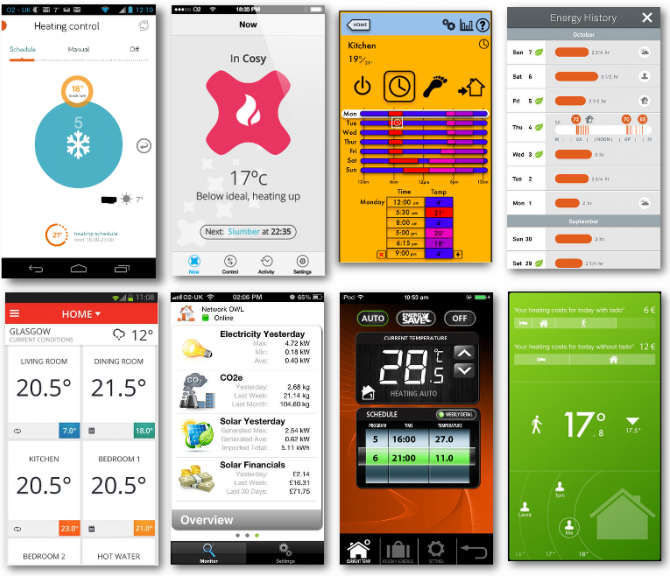
\includegraphics[width=0.8\textwidth]{images/smart_heating_apps.png}
	\end{center}
	\caption{Some examples of mobile applications for controlling smart heatings systems. Source: \url{https://cdn.recombu.com/media/digital/news/legacy/M13058/1397569835_w670_h576.png}}
	\label{fig:smart_heating_apps}
\end{figure}


\section{Use Cases}

We started by analyzing different use cases that an average user might run into while using a smart heating system. This way we were able to ensure that our design decision would lead to a simple yet effective application which helps the user control the system in a simple manner without overcomplicating things. There is a tradeoff that certain functionality might be lost because of these decisions but our main focus was to create an application which is easy to use. 

\begin{enumerate}
\item \textbf{Use Case: User wants to install the system}

The user is presented with a welcome screen explaining how he can setup his smart heating system. Via a simple scan of the NFC tag on the raspberry pi, the user is registered on the server and is ready to add new rooms to his system.
\item \textbf{Use Case: User wants to add a room to the system}

After installation the user will start in the home screen (see Section X) upon opening the application. Through the menu located in the top bar the user can then select "Add a new room". After successful addition of a room the application will switch to the detailed view of the new room (see Section Y).
\item \textbf{Use Case: User wants to add a thermostat to a room}

From the home screen the user can select any room from the system to get to the detailed view of the room. Through the menu located in the top bar the user can then select "Add a new thermostat".
\item \textbf{Use Case: User wants to setup the heating schedule for a room}

From the home screen the user can select any room from the system to get to the detailed view of the room. Through the menu located in the top bar the user can then select "View schedule". This will open the schedule view (see Section Z) in which the user can easily change the existing heating schedule by simply selecting the desired day and time in the view. He can also choose the option to replace all entries with an existing heating schedule from a different room via the menu from the top bar.
\item \textbf{Use Case: User wants to change the current temperature in a room}

From the home screen the user can select any room from the system to get to the detailed view of the room. The detailed view shows the current temperature as well as the current desired temperature according to the room's heating schedule. Using the slider on the right side the user can easily change the desired temperature for this room.

\item \textbf{Use Case: User wants to }

From the home screen the user can select any room from the system to get to the detailed view of the room. The detailed view shows the current temperature as well as the current desired temperature according to the room's heating schedule. Using the slider on the right side the user can easily change the desired temperature for this room.
\end{enumerate}

\subsection{Evaluation}

Uses cases 5 and 8 are neglected because of reasons.... Evaluate the use cases, explain what was solved and what wasn't and why it wasn't.

\section{Application flow}
\begin{figure}[h]
\begin{tikzpicture}
    % Place nodes
    \node [block] (welcome) {Welcome View};
    \node [block, right of=welcome, node distance = 3cm] (home) {Home View};
    \node [block, right of=home, node distance = 5cm] (room) {Room Detail View};
    \node [block, right of=room, node distance = 5cm] (schedule) {Schedule View};
    % Draw edges
    \path [draw=black,solid,line width=1mm,preaction={-triangle 90,thin,draw,shorten >=-0.5mm}] (home) -- ([yshift=-1cm]home.south) -- ([yshift=-1cm]room.south)  node [midway, above]{Add new room} -- (room.south) ;
    \path [draw=black,solid,line width=1mm,preaction={-triangle 90,thin,draw,shorten >=-0.5mm}] (welcome) -- (home);
    \path [draw=black,solid,line width=1mm,preaction={-triangle 90,thin,draw,shorten >=-0.5mm}] (home) -- (room) node [midway, above] {Select Room};
    \path [draw=black,solid,line width=1mm,preaction={-triangle 90,thin,draw,shorten >=-0.5mm}] (room) -- (home) node [midway, below] {Back};
    \path [draw=black,solid,line width=1mm,preaction={-triangle 90,thin,draw,shorten >=-0.5mm}] (room) -- (schedule) node [midway, above] {Edit Schedule};
    \path [draw=black,solid,line width=1mm,preaction={-triangle 90,thin,draw,shorten >=-0.5mm}] (schedule) -- (room) node [midway, below] {Back};
\end{tikzpicture}
\caption{The application flow of the mobile app.}
	\label{fig:app_flow}
\end{figure}
